\documentclass[a4paper]{article}

%% Language and font encodings
\usepackage[english]{babel}
\usepackage[utf8x]{inputenc}
\usepackage[T1]{fontenc}

%% Sets page size and margins
\usepackage[a4paper,top=3cm,bottom=3cm,left=3cm,right=3cm,marginparwidth=1.75cm]{geometry}

%% Useful packages
\usepackage{amsmath}
\usepackage{graphicx}
\usepackage{caption}
\usepackage{subcaption}
\usepackage{url}
\usepackage{enumitem}


\title{Tracking Multiple Objects From Partial Observations}
\author{Chinmayee Shah}
%\date{}

\newcommand{\N}{\mathcal{N}}
\newcommand{\x}{\hat{x}}
\newcommand{\X}{\hat{X}}
\newcommand{\y}{\hat{y}}
\newcommand{\Y}{\hat{Y}}
\newcommand{\dt}{\text{dt}}

\begin{document}
\maketitle

\section{Problem}

Reliable object detection, tracking, and trajectory prediction is of great
interest today, for safe autonomous navigation.
This project explores the problem of tracking multiple objects, given
noisy observed object positions.
Sensors such as lidar and radar can see what is directly in front of them,
but they cannot see occluded objects.
Lidar sensors scan their environment, and record the distance to
nearest objects, as a list of \{angle, distance\} pairs.
The recorded distance can be noisy due to sensor noise, scattering and
partial and multiple reflections.

In this project, we look at the problem of tracking objects given a set of
observed positions for objects, using Bayesian inference and maximum 
likelihood.
Given a set of $M(\tau)$ observations,
$\X_\tau = \{\x^\tau_1, \x^\tau_2, \ldots, \x^\tau_{M(\tau)}\}$,
for $N(\tau)$ objects ($M(\tau) \leq N(\tau)$ because of occlusion),
for times $\tau \leq t$,
we would like to estimate $N(t)$, that is, how many objects there
really are at time $t$, and true positions of all objects at time $t$, that is,
$X_t = \{x^t_1, x^t_2, \ldots, x^t_{N(t)}\}$.
We do this by choosing the most likely association between observations and
existing objects, creating new tracks for observations that are likely from
newly entered objects, deleting tracks that have likely exited or were
spuriously created in the past, and
evolving and refining track estimates using previous estimates and new
observations, as in a hidden Markov process.


\section{Literature Review}

Typically, one must first pre-process raw lidar data to detect objects and
estimate their positions.
These observed positions can then be used to track objects.
Globally nearest neighbors,
probabilistic data association filtering (PDAF) and joint probabilistic data association
filtering (JPDAF) all assume that pre-processing is done, and final observed positions have
been computed~\cite{pdaf}.
Globally nearest neighbors (GNN) weights each observation to track association by a score,
and either locally or globally tries to maximize this weight.
PDAF assigns probabilities to all matches, and updates estimates using these probabilities
as weights -- that is, it does not pick a best association, but uses all observations to
update the estimate.
PDAF may falsely assign one observation to multiple tracks. JPDAF overcomes this by
conditioning over only valid assignments.
PDAF and JPDAF are known to be computationally expensive.
Moreover, they assume the number of tracks is known.
Markov chain Monte Carlo data association provides a polynomial randomized approximation
scheme for joint probabilistic data association~\cite{mcmcda}.
The problem model for these algorithms is slightly different from ours --
they look at clutter, where there may be false alarms from each track, so that there
may be multiple observations per track.
In our problem, we have at most one observation per track.
Multi-hypothesis is similar to globally nearest neighbors, but across multiple time
steps~\cite{mht}. It tracks multiple hypothesis (associations) in the hope that
information from future steps will provide more information.
In concept, it is similar to beam search.

End-to-end approaches~\cite{deeptracking} on the other hand, use a stack of
convolutional neural networks and recurrent neural networks to track objects
directly from sensor data.
However, this provides little insight into how the network is performing tracking,
and requires training on huge data-sets.
It is also not clear how a network trained on one kind of data set would perform on
another kind of data set.
In this project, we take a more intuitive approach of Bayesian networks,
assume we have observed positions, and look at the problem
of just estimating true positions of objects given observed positions.


\section{Data and Task}

There are many lidar point cloud data-sets publicly available.
However, we cannot directly use these data-sets -- we need to pre-process
the data to detect objects and estimate positions, which in itself is a
challenging problem.
Also, these real-world data-sets do not include true number of objects,
or true positions of objects, making evaluation and error estimation
difficult.
We generate synthetic data by evolving objects using a 2D simulation, and
record true and observed positions of each object, and whether an object
is visible or occluded.
Generating data using simulation also  lets us break the problem of object
tracking into smaller, more manageable problems.

\begin{figure}[t]
  \centering
  \begin{subfigure}{0.48\textwidth}
  \centering
  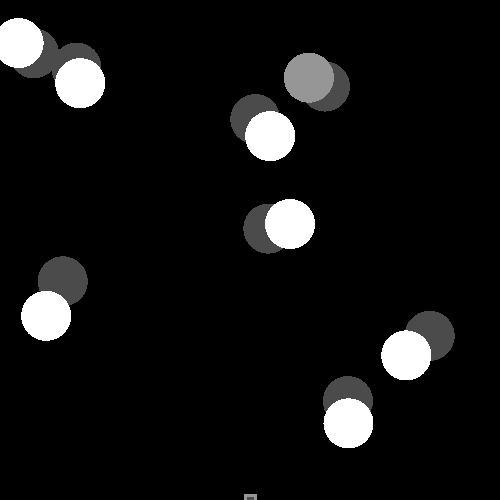
\includegraphics[width=0.6\textwidth]{images/input_1.png}
  \end{subfigure}~
  \begin{subfigure}{0.48\textwidth}
  \centering
  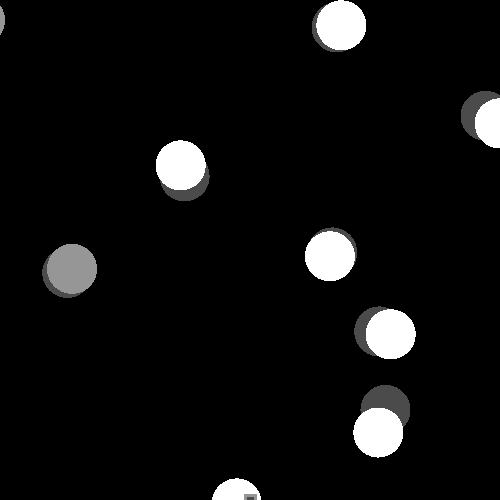
\includegraphics[width=0.6\textwidth]{images/input_2.png}
  \end{subfigure}
  \caption{Two frames from data generated using a simple 2D simulation.
           White shows true position for visible objects,
           light gray shows true position for occluded objects,
           dark gray shows noisy position (when an observation is used).}
  \label{fig:input}
\end{figure}

\subsection{Simulation setup}

The simulation domain is a rectangular region, with a viewer at the center
of the bottom edge, denoted by the gray square in figure~\ref{fig:input}.
White circles are objects visible to the viewer, and light gray circles
are occluded objects not visible to the viewer
(circle center gives object position).
The simulator evolves objects at each step using the equations of motion
$x_{t} = u_{t-1} \delta t + \frac{1}{2} a_{t-1} \delta t^2 $ and
$u_{t} = u_{t-1} + a_{t-1} \delta t$, where $x_t$, $u_t$ and $a_t$ denote
the position, velocity and acceleration at time $t$ and $\delta t$ is a
constant time step.
The observed position equals true position plus noise.
Acceleration and noise are independent and identically distributed random
variables, drawn from normal distributions
$\N(0, \Sigma_a)$ and $\N(0, \Sigma_r)$ respectively,
where
$\Sigma_a = \begin{bmatrix} \sigma_a^2 & 0 \\ 0 & \sigma_a^2 \end{bmatrix}$
and
$\Sigma_r = \begin{bmatrix} \sigma_r^2 & 0 \\ 0 & \sigma_r^2 \end{bmatrix}$.
Dark gray circles in figure~\ref{fig:input} denote noisy positions,
which are observed positions for visible objects.
The simulator generates a new object with a probability $p_\text{gen}$ at
each step, if the number of objects is less than $N_\text{max}$ and 
greater than $\frac{N_\text{max}}{2}$, and with probability 1 if
the number of objects is less than $\frac{N_\text{max}}{2}$. The total
number of objects thus never exceeds $N_\text{max}$.
The simulator initializes a new object with a position drawn uniformly from
points along the boundary of the simulation region, and with a velocity $\mu_v$
towards the opposite edge.
Objects outside the simulation region are deleted.

At each step, the simulator records the total number of objects, object id,
the true and observed position of each object, and whether the object is
occluded or visible to the viewer at the bottom.

\subsection{Task}

Given a set of $M(\tau)$ observations,
$\X_\tau = \{\x^\tau_1, \x^\tau_2, \ldots, \x^\tau_{M(\tau)}\}$,
for $N(\tau)$ objects ($M(\tau) \leq N(\tau)$), for times $\tau \leq t$,
we want to estimate the true number of objects $N(\tau)$ and true positions $X_t$.
We assume we know the distribution for acceleration and noise, that is, they are i.i.d.,
and drawn from normal distributions $\N(0, \Sigma_a)$ and $\N(0, \Sigma_r)$, and that
objects evolve according to the equations of motion presented in the previous section.


\section{Approach}

Estimating $N(t)$ and $X_t$ given $\X_1, \X_2, \ldots, \X_t$ is difficult, because
observations are noisy, that is, they do not correspond to true positions,
we do not know which observations correspond to which objects, and
some observations might be missing and we not know how many objects there 
really are -- new objects might have entered, and existing objects might have exited.
We solve the problem by looking at three smaller problems --
first, estimating true positions of objects at time $t$ given noisy positions
(observations) for all objects, including occluded objects, and association between 
observations and objects till time $t$,
second, determining an association between observations and objects given all
observations
and finally, determining an association between observations and objects given
observations for only visible objects.

\subsection{Tracking objects from noisy positions given association}

The true position and velocity of each object at a time $t$ depends only on 
the true position, velocity and acceleration of object at time $t-1$.
\begin{figure}[h]
  \centering
  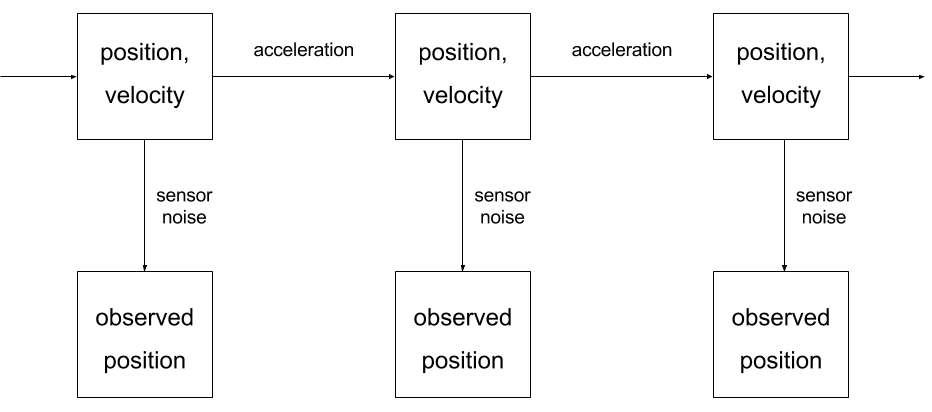
\includegraphics[width=0.6\textwidth]{images/hmm.png}
  \caption{Future position depends only on current position and velocity,
  for each object.}
  \label{fig:HMM}
\end{figure}
We can think of position and velocity of each object as states of a hidden Markov
process, and the observed positions as the observed states of this process.
Figure~\ref{fig:HMM} illustrates this.

Given the past and current observed positions for each object, we can recursively
estimate the probabilities of unknown, hidden state using observations as they come,
using Bayesian inference.
Kalman filter recursively computes an estimate for state and its covariance at
time $t$ using state estimate at time $t-1$ (predict phase),
and then refines the estimate using observation at time $t$, given
process noise and observation noise distribution~\cite{kalman}.
Since process noise (acceleration) and observation noise are normal in our case,
these estimates yield the exact probability distributions for state estimates for
each object, and maximize posterior probability.

We use Kalman filter to estimate each object's hidden state (position and velocity)
and state covariance, given all observations, and association between observations
and objects.
The hidden state $y$ for each object comprises of position $x$ and velocity $v$,
$y = \begin{bmatrix} x & v \end{bmatrix}$.
Observed positions are denoted by $\x$, true positions by $x$, and estimated
state mean by $\y$.
The velocity $v$ is not observed, and hence, observed state equals $\x$.
For each object, Kalman filter predicts state at step $t$ as follows,
\begin{align*}
\y_{t|t-1} &= F \y_{t-1|t-1} \\
P_{t|t-1}  &= F P_{t-1|t-1} F^T + Q
\end{align*}
Here, the matrix $F$ gives how state evolves, and equals
$\begin{bmatrix} I & I \cdot \dt \\ 0 & I \end{bmatrix}$.
The matrix $Q$ denotes process noise, and is related to acceleration,
$Q = G G^T \sigma_a^2$, where
$G = \begin{bmatrix} \frac{1}{2} \cdot I \cdot \dt^2 & I \cdot \dt \end{bmatrix} ^T$.
$I$ is a $2 \times 2$ identity matrix, and $0$ is a $2 \times 2$ matrix
with all elements set to zero.
The update phase uses a new observation at time $t$, to refine the estimates as,
\begin{align*}
z_t        &= \x_t - H \y_{t|t-1} \\
S_t        &= H P_{t|t-1} H^T + R \\
K_t        &= P_{t|t-1} H^T S^{-1} \\
\y_{t|t}   &= \y_{t|t-1} + K_t z_t \\
P_{t|t}    &= (I - K_t H) P_{t|t-1}
\end{align*}
The matrix $H$, the observation matrix, transforms the hidden state $y$ to what is observed.
Since only the object position is observed, $H = \begin{bmatrix} I & 0 \end{bmatrix}$.
$R = \Sigma_r$ is the observation noise.
An actual observation $\x = H y + r$, where $r$ is a noise value and $y$ is the true state.

The estimated state $\y$ is the maximum a posteriori (MAP) estimate.
By running Kalman filter on each object, we thus get the MAP estimate for the position
and velocity of each object.

\subsection{Associating objects given all observations (no occlusion)}

Once we have associations between object tracks and observations, we can use Kalman
filter to estimate the true positions of objects.
But we only have a set of observed positions and we need to determine the association
between observations and tracks first.
In this part, we assume that we have exactly one noisy observation for every object.
With this setup, we know that the number of object tracks must be equal to the number
of observations, that is $N(t) = M(t)$.
One approach is to match the nearest objects and observations.
However, greedily matching nearest object to an observation may not be optimal globally,
as there might be clusters of nearby objects.
Also, the greedy approach cannot be extended to the case when observations might be
missing due to occlusion.
Finally, even though $N(t)$ equals $M(t)$, $M(t)$ does not necessarily equal $M(t-1)$
as tracks enter and leave the domain.
We compute a penalty/loss for each object-observation match, and for unmatched tracks
and observations, and select the association that gives the least total loss.
To limit the search
(there would be more than $N(t)!$ associations if we were to include all possible
matches with tracks entering and leaving),
we include only those tracks that are within a small distance from an observation
(gate tracks), when determining a track to match.
We experimented with 2 different loss functions --
the distance between track position and observation, and
negative log of the probability that an observation is from a track,
assuming the estimated track position is the true position.
The ideas of gating and computing scores for association are inspired by
globally nearest neighbors and multi-hypothesis tracking~\cite{mht}.
We choose the best association unlike JPDAF which uses all observations weighted by
probability, to evolve a track, because in our problem, we assume there
is no clutter, and each track has at most one observation (no false alarms).

\subsubsection{Distance based loss}
For an object-observation pair, the loss equals the Euclidean distance between them.
For an unmatched observation pair, we assume that it must be a new track, and take
the least distance to the boundary as the loss, thus heavily penalizing unmatched
observations near the center. Unmatched observations near the boundary are penalized
less. Similarly, for an unmatched track, we assume it must have left the domain,
and take the least distance to boundary as the loss.

\subsubsection{Maximum likelihood formulation}
For an object-observation pair, the loss in this case equals negative of log of
probability that the observation is from a track, assuming the current estimate of
track as the actual position.
We discretize the PDF and approximate probabilities as $\text{PDF} \times \Delta$,
to approximate the probability for new and leaving tracks.
For an observation-track pair, this translates to
$-\log(P_\N(x_{t|t-1}, \Sigma_r, \x_t)) \Delta$,
where $x_{t|t-1}$ is our MAP estimate of position at time $t$ given previous
observations, that is,
$H \y_{t|t-1}$,
$\Sigma_r$ is observation noise, $\x_t$ is observation at time $t$,
$P_\N(\mu, \Sigma, x))$ is normal PDF with mean $\mu$,
covariance $\Sigma$, evaluated at $x$, and $\Delta$ is size of discretization.
For an unmatched observation, the loss equals
$- \sum_{x'} \log(P_\N(x', \Sigma_r, \x_t)) \Delta$, where the sum is over
points $x'$ outside the rectangular region.
We limit the sum till $4\sigma_r$ on each side of $x_{t|t-1}$.
Similarly, for an unmatched track, the loss equals
$- \sum_{x'} \log(P_\N(x_{t|t-1}, \Sigma_r, x')) \Delta$.

\subsubsection{Algorithm}
The algorithm for estimating positions given a set of noisy positions, but
no missing objects, looks as follows:
\begin{enumerate}[itemsep=0mm]
\item Predict position for tracks at time $t$, using estimated positions at time $t-1$.
\item For each observation, find tracks that are within a small region around the 
observation
(an axis aligned box $10 (\sigma_a + \sigma_r)$ long in each dimension,
centered at the observation, in our experiments)
\item Search for the association that gives the least loss (penalty).
Total loss for an association =
  $\Sigma_{a \in A}$ loss for matching $a.$track and $a.$observation +
  $\Sigma_{c \in C}$ penalty for creating a new track for observation $c$ +
  $\Sigma_{d \in D}$ penalty for deleting track $d$.
$A$ is the set of matched observation-track pairs, $C$ is unmatched observations, and
$D$ is unmatched tracks.
\item Use the association from previous step to update the estimate for each track in $A$, create new tracks for observations in $C$ and delete tracks in $D$.
\end{enumerate}


\subsection{Handling missing observations and occlusion}

In this part, we look at the case when observations for occluded objects are missing.
Here, $N(t)$ is not necessarily equal to $M(t)$. We extend the maximum likelihood
formulation in the previous section, so that an unmatched track may either be occluded,
or may be outside the rectangular region (and should be deleted).
When a track is unmatched, but is occluded, we use the predict equations of Kalman filter
to evolve the object track, and skip the update part, where an observation is used to
refine the estimate.

\subsubsection{Maximum likelihood formulation}
Loss for object-observation pair and unmatched observation is same as the unoccluded case.
Loss for unmatched track now has two components --
outside points and occluded points, \\
$- \sum_{x' \in \text{outside}} \log(P_\N(x', \Sigma_r, \x_t)) \Delta - \sum_{x' \in \text{occluded}} \log(P_\N(x', \Sigma_r, \x_t)) \Delta$, \\
where outside is points outside the rectangular region,
and occluded is points that seem occluded to the viewer.
Points that seem occluded to the viewer are not the same as points that are actually
occluded, as observed positions are noisy.
We compute observed occluded region for every step by tracing rays from viewer to each
point in the domain, and checking if the ray crossed an observed object
(assuming objects are circular with some finite radius).

A more complete formulation should also consider the prior probability distribution
on track estimates.
This can be computed using the state mean and covariance from Kalman filter.
We experimented with this formulation too, and got similar results, but the formulation
is computationally more expensive -- we can compute and cache discretized
probabilities $P_\N(0, \Sigma_r, x-\mu)$ for the former case,
but we need to compute the probabilities in the latter case every time.

\subsubsection{Deleting spurious tracks}
We noticed that sometimes, we have falsely created tracks, especially at the boundary
when objects are just entering, and when the probability that an observation corresponds
to a new track is high. That is, we falsely get multiple tracks for just one object.
These clusters of false tracks keep moving through the domain, even though there is really
just one object.
We delete tracks that are in visible region, but do not match to any observation for some
number of consecutive frames, to avoid such spurious tracks.
We did not face this issue in the previous problem where we had all observations, because
we knew $N(t)$ then, and limited search to cases where number of tracks equals number of observations.

\subsubsection{Algorithm}

The final algorithm for tracking objects from partial observations is:
\begin{enumerate}[itemsep=0mm]
\item Predict position for tracks at time $t$, using estimated positions at time $t-1$.
\item For each observation, gate tracks to a small region around the observation as before.
\item Search for association that gives least total loss, where the total loss now includes
the probability that an unmatched track is occluded and hence not observed.
\item Create new tracks for unmatched observations, and delete tracks outside the domain,
and those that seem spurious.
\item Update estimates for tracks that have a matching observation.
\end{enumerate}


\section{Implementation and Results}
We have implemented the simulation and all discussed algorithms in python, our code is
available at \url{https://github.com/schinmayee/bayesian-object-tracking}.
We have also included the code and results in a codalab worksheet at
\url{https://worksheets.codalab.org/worksheets/0xee9369450dfa40f8a006a2f54da38876/}.
Estimated positions are saved as images such as images here, in results
folder for each run, on the codalab sheet.

\begin{figure}[h]
  \centering
  \begin{subfigure}{0.48\textwidth}
  \centering
  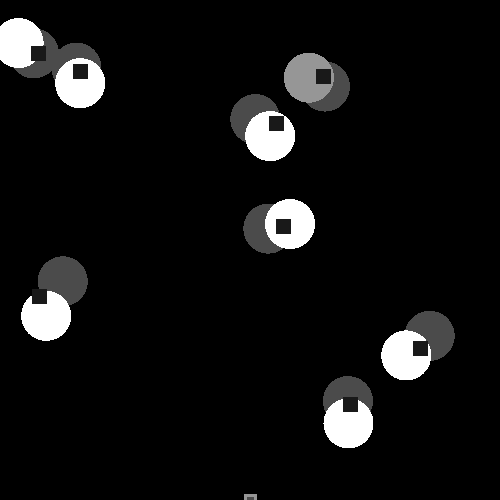
\includegraphics[width=0.6\textwidth]{images/kalman_1.png}
  \end{subfigure}~
  \begin{subfigure}{0.48\textwidth}
  \centering
  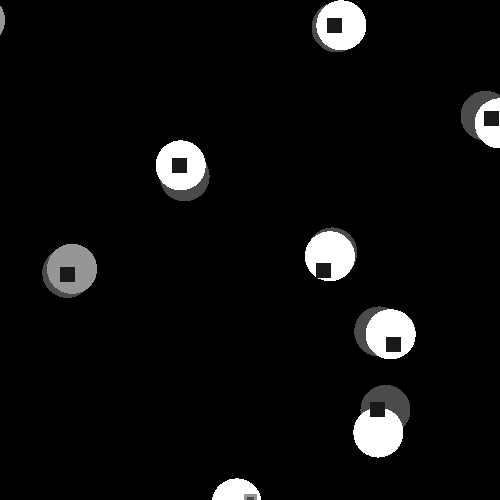
\includegraphics[width=0.6\textwidth]{images/kalman_2.png}
  \end{subfigure}
  \caption{Estimates using Kalman filter, given association.}
  \label{fig:kalman}
  \vspace{-2pt}
\end{figure}
\begin{figure}[h]
  \centering
  \begin{subfigure}{0.48\textwidth}
  \centering
  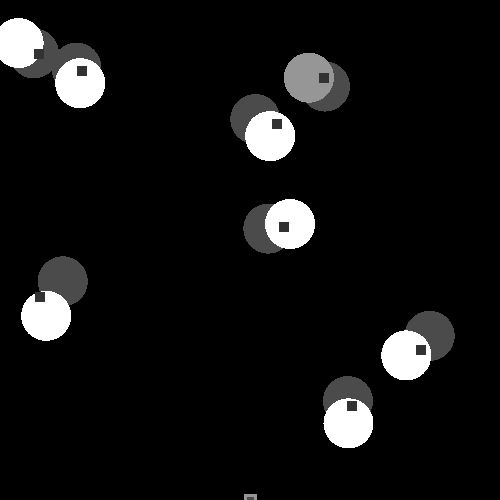
\includegraphics[width=0.6\textwidth]{images/nearest_1.png}
  \end{subfigure}~
  \begin{subfigure}{0.48\textwidth}
  \centering
  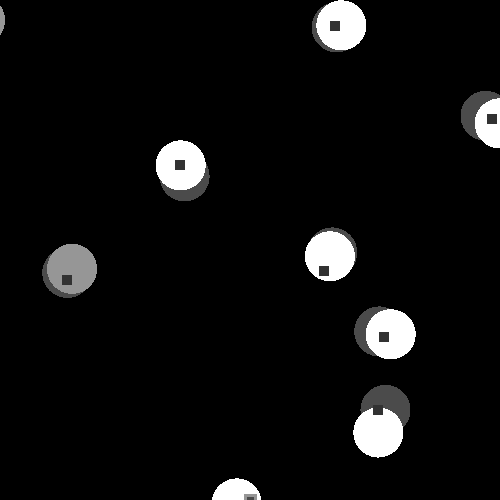
\includegraphics[width=0.6\textwidth]{images/nearest_2.png}
  \end{subfigure}
  \caption{Estimates using Euclidean distance as loss.}
  \label{fig:nearest}
  \vspace{-2pt}
\end{figure}

Figure~\ref{fig:kalman} shows results for 2 frames for the first part,
estimating position using Kalman filter, when all observations are available,
and the association is also given.
Light gray and white circle centers give true positions, and dark gray circle
centers give observed positions. Dark gray squares are the estimated positions.
Kalman filter seems to work quite well, even when observations are very noisy,
such as the circle in the middle on the left, in the left figure -- the estimate
lies in the white region, even when the gray region (noise) is almost outside
the white region.
Kalman filter gives the MAP estimate, and uses previous estimate of the state
to effectively reduce the observation noise.

Figure~\ref{fig:nearest} shows results for the same frames for second part,
determining association between objects and observations and estimating
positions, given all observations.
It uses Euclidean distance between observation and track estimate as loss function.
The estimates seem to be very close to estimates given by Kalman filter.
Figure~\ref{fig:unoccluded_ml} shows results for the same setup, with
negative log probability as the loss function. These results look similar
to the distance based loss function.
However, this algorithm falsely creates, in the second frame, a new track for
the circle at top right -- bigger squares denote newly created tracks and
smaller squares denote old tracks.
The probability that the observation is a new track and the old track has left
seems to be more than the probability that the observation is from an old track.
The distance loss function also runs into this problem, but less often.
\begin{figure}[h]
  \centering
  \begin{subfigure}{0.48\textwidth}
  \centering
  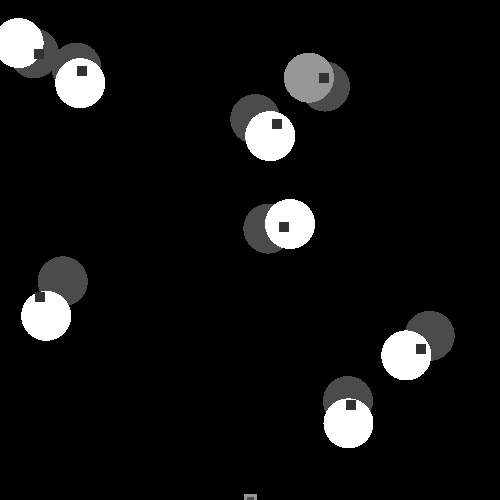
\includegraphics[width=0.6\textwidth]{images/unoccluded_ml_1.png}
  \end{subfigure}~
  \begin{subfigure}{0.48\textwidth}
  \centering
  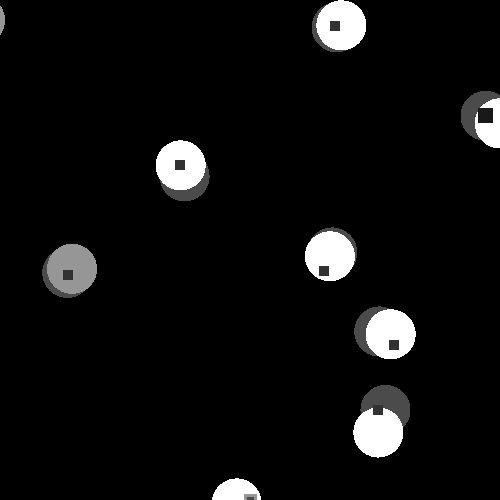
\includegraphics[width=0.6\textwidth]{images/unoccluded_ml_2.png}
  \end{subfigure}
  \caption{Estimates using negative log probability as loss.}
  \label{fig:unoccluded_ml}
  \vspace{-2pt}
\end{figure}

Figure~\ref{fig:occluded_ml} shows results for the final part, where
observations for occluded objects are missing, and association is unknown.
Light gray circles denote occluded objects.
The frame on right shows some spurious tracks created near the boundary --
there are two false tracks in the left corner, and one falsely created new
track resulting in one stray track along the right edge.
However, the algorithm does seem to track occluded objects correctly in 
most cases, particularly in the interior.
\begin{figure}[h]
  \centering
  \begin{subfigure}{0.48\textwidth}
  \centering
  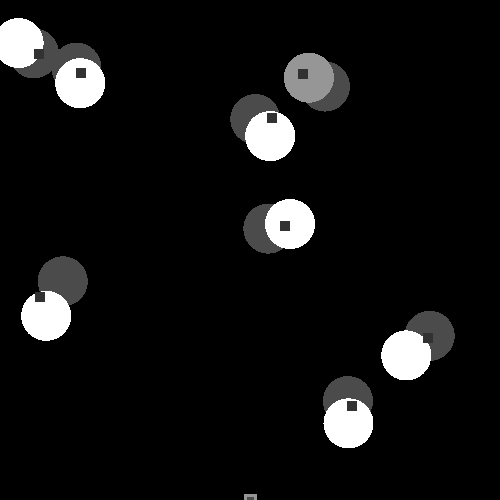
\includegraphics[width=0.6\textwidth]{images/occluded_ml_1.png}
  \end{subfigure}~
  \begin{subfigure}{0.48\textwidth}
  \centering
  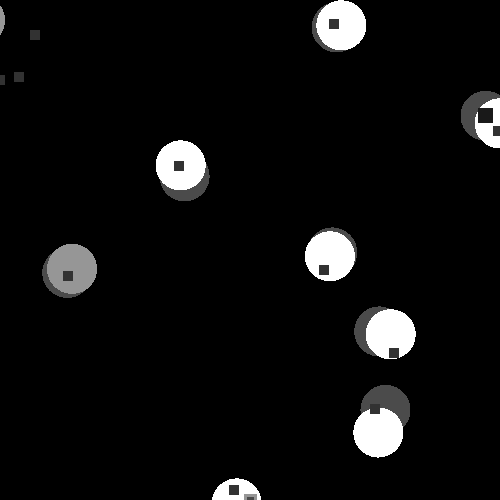
\includegraphics[width=0.6\textwidth]{images/occluded_ml_2.png}
  \end{subfigure}
  \caption{Estimates when observations for occluded objects are missing}
  \label{fig:occluded_ml}
  \vspace{-2pt}
\end{figure}

For the cases where association information is not available, we find that
false new tracks are sometimes created near the boundary, as in
figure~\ref{fig:unoccluded_ml} and figure~\ref{fig:occluded_ml}.
As objects move closer to the center, they are tracked more accurately, even
in the occluded object case, as the penalty for creating new tracks in the
interior is high.
\begin{figure}[h]
  \centering
  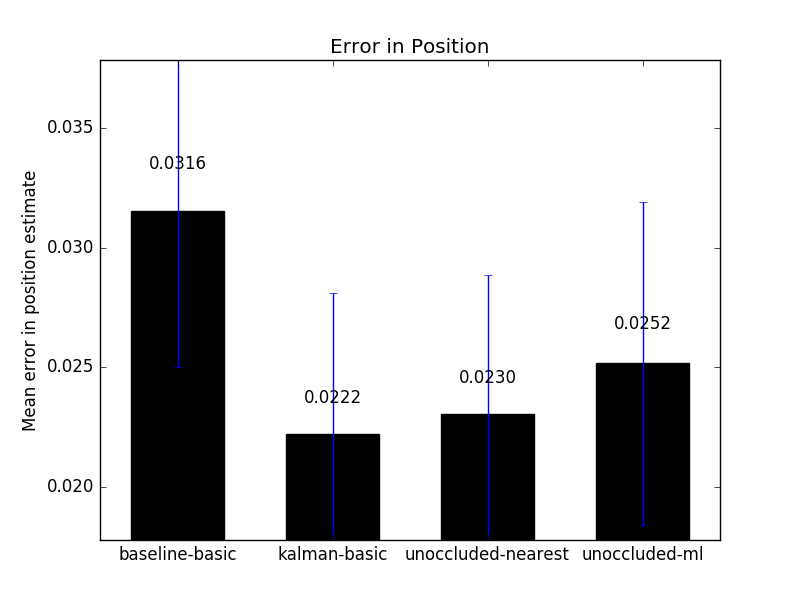
\includegraphics[width=0.6\textwidth]{images/position_error.png}
  \caption{Error in position, averaged over 100 frames.}
  \label{fig:errors}
\end{figure}
Figure~\ref{fig:errors} shows error in estimated position for 4 cases.
The first bar, baseline-basic is the observation error, if observations for
all objects are available, and we use the observed position as the position estimate.
The second one, kalman-basic, gives the estimation error for Kalman
filter, given all observations and association. Kalman filter reduces error over
baseline by 1.4x. The next two bars give errors when all observations are
available, but association information is not. As expected, both errors are more
than kalman-basic. Somewhat surprisingly, both errors are still less than
baseline-basic, even without the association information, and the error for
the probabilistic formulation is more than the one with distance based loss.

We think that we get more false tracks with the probabilistic formulation,
as compared to distance as the loss function, because,
with the probabilistic formulation, we have more false tracks at the boundaries,
when it is likely that an observation is from a new
track, as a result of which the estimation error equals observation error at
the boundaries.
The probabilistic formulation adds up probability for a new track,
from all points on and outside the boundary, while the distance based loss
only takes the least distance to boundary as loss.
This means it is better to create new tracks at the boundary, in the probabilistic
formulation.
Moreover, since we use Euclidean distance rather than squared Euclidean distance
for distance loss, small distances from the boundary get a larger penalty, compared
to negative log probability, which will have squared distance in the numerator
since the probability is for a normal distribution.
If we factored in the probability that there is a new object at the boundary
(using the average rate at which new objects are created), then the formulation
would be more complete, and probably give better results,
as the probability of a new track would become smaller, and the corresponding
negative log would become larger.
This argument also extends to the case with occlusion, when observations are missing.

Finally, we do not have an error bar for the last case, where observations
are missing, as estimation error no longer makes sense when we have false
tracks. Instead, we have the results for 40 frames, on Codalab, that shows
estimated track positions.


\section{Discussion, Conclusion, Future Directions}

The problem of multiple object tracking has rich literature, with
techniques such as multi-hypothesis tracking, probabilistic data association
filter, and joint probabilistic data association filter.
However, many of these formulations assume that the number of tracks is known.
End-to-end deep tracking is a novel approach that uses a stack of convolutional
neural networks and recurrent neural networks to perform tracking using sensor
data~\cite{deeptracking}.
We tried a different approach in this project, using Bayesian networks.
While the results look great without occlusion, we get some false tracks at
boundaries.
We think if we factor in the probability of new objects, the rate at which
we get false tracks should go down.
Even with the current formulation, tracking is robust in the interior.
In a realistic case, an observer is probably at the center, with a $360^o$
view, and making a few errors for tracks far away, that are just entering the 
field of view, is probably not bad.

Our approach requires assumptions about the distribution of process and
observation noise, and how system evolves.
As an interesting future direction,
it might be possible to learn some of this so that we can make fewer 
assumptions about distribution of observation noise, process noise,
and even how the system evolves.
This might be useful in scenarios such as road intersections, round-abouts,
curved roads, where traffic tends to move in a certain way.

\pagebreak

\bibliography{paper}{}
\bibliographystyle{plain}

\end{document}